% https://tex.stackexchange.com/a/442370
\documentclass{beamer}
\usepackage[utf8]{inputenc}
\usepackage{subfiles}
\usepackage{circuitikz}
\usepackage{tikz}
\usetikzlibrary{arrows,shapes.gates.logic.US,shapes.gates.logic.IEC,calc}
\usetikzlibrary{overlay-beamer-styles} %<-added


\usecolortheme{orchid}

\begin{document}
\begin{frame}

\setbeamercovered{dynamic}

\centering
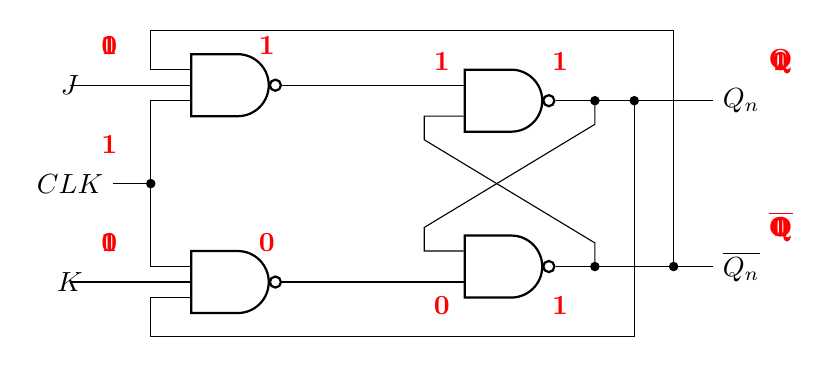
\begin{tikzpicture}
%\draw (0,0) rectangle (9,5); % Use this to set the dimensions to approximately the page size

        \node(J) at (1,0) {$J$};
        \node[nand gate US,draw,logic gate inputs = nnn,thick] at ($(J)+(2,0)$) (Nand1){};

        \node(K) at ($(J)+(0,-2.5)$) {$K$};
        \node[nand gate US, draw, logic gate inputs = nnn,thick] at ($(K)+(2,0)$) (Nand2) {};

        \node[nand gate US, draw, logic gate inputs = nnn, thick,anchor=input 1] at ($(Nand1)+(3,0)$) (Nand3) {};
        \node[nand gate US, draw, logic gate inputs = nnn, thick, anchor = input 3] at ($(Nand2)+(3,0)$) (Nand4) {};

        \draw(J) |- (Nand1.input 2);
        \draw(K) |- (Nand2.input 2);
        \path (J) -- (K) node[midway] (CLK) {$CLK$};

        \draw (Nand1.input 3) --++(180:5mm) coordinate (aux) |- (CLK);
        \draw (CLK-|aux)|- (Nand2.input 1);

        \draw(Nand1.output) |- (Nand3.input 1);
        \draw(Nand2.output) |- (Nand4.input 3);

        \draw (Nand3.output) -- ([xshift=2cm]Nand3.output);
        \draw (Nand4.output) -- ([xshift=2cm]Nand4.output);

        \draw (Nand3.output) --++(0:2cm) node[right](Q) {$Q_n$} coordinate[pos=.25] (aux1) coordinate[pos=.5] (aux2);
        \draw (Nand4.output) --++(0:2cm) node[right] (QN) {$\overline{Q_n}$} coordinate[pos=.25] (aux3) coordinate[pos=.75] (aux4);

        \node[visible on=<{2}>](out1) at ($(Q)+(0.5,0.5)$) {\textcolor{red}{\textbf{Q}}};

        \node[visible on=<{3}>](out1) at ($(Q)+(0.5,0.5)$) {\textcolor{red}{\textbf{0}}};
        \node[visible on=<{4}>](out1) at ($(Q)+(0.5,0.5)$) {\textcolor{red}{\textbf{1}}};
       % \node[visible on=<{5}>](out2) at ($(Q)+(0.5,0.5)$) {\textcolor{red}{{$\overline{\textbf{Q}}$}}};

       \node[visible on=<{2}>](out2) at ($(QN)+(0.5,0.5)$) {\textcolor{red}{{$\overline{\textbf{Q}}$}}};

       \node[visible on=<{3}>](out2) at ($(QN)+(0.5,0.5)$) {\textcolor{red}{\textbf{1}}};
       \node[visible on=<{4}>](out2) at ($(QN)+(0.5,0.5)$) {\textcolor{red}{\textbf{0}}};

        \node[visible on=<{2,3}>](in1) at ($(J)+(0.5,0.5)$) {\textcolor{red}{\textbf{0}}};
        \node[visible on=<{4}>](in1) at ($(J)+(0.5,0.5)$) {\textcolor{red}{\textbf{1}}};

        \node[visible on=<{2,4}>](in2) at ($(K)+(0.5,0.5)$) {\textcolor{red}{\textbf{0}}};
        \node[visible on=<{3}>](in2) at ($(K)+(0.5,0.5)$) {\textcolor{red}{\textbf{1}}};

        \node[visible on=<{5,6,7,9}>](in1) at ($(J)+(0.5,0.5)$) {\textcolor{red}{\textbf{1}}};
         \node[visible on=<{5,6,7,9}>](in2) at ($(K)+(0.5,0.5)$) {\textcolor{red}{\textbf{1}}};

         \node[visible on=<{6,7,8}>](out1) at ($(Q)+(0.5,0.5)$) {\textcolor{red}{\textbf{1}}};
         \node[visible on=<{6,7,8}>](out1) at ($(QN)+(0.5,0.5)$) {\textcolor{red}{\textbf{0}}};

         \node[visible on=<{6,7,9}>](out1) at ($(CLK)+(0.5,0.5)$) {\textcolor{red}{\textbf{1}}};

%         \node[visible on =<{6}>]  at($(CLK)+(4,-4)$) {\text{CLK IS 1}};

         \node[visible on=<{7,8}>](out1) at ($(Nand1)+(0.5,0.5)$) {\textcolor{red}{\textbf{1}}};
         \node[visible on=<{7,8}>](out1) at ($(Nand2)+(0.5,0.5)$) {\textcolor{red}{\textbf{0}}};

          \node[visible on=<{8}>](out1) at ($(Nand3)+(-0.75,0.5)$) {\textcolor{red}{\textbf{1}}};
           \node[visible on=<{8}>](out1) at ($(Nand4)+(-0.75,-0.5)$) {\textcolor{red}{\textbf{0}}};

            \node[visible on=<{9}>](out1) at ($(Nand3)+(0.75,0.5)$) {\textcolor{red}{\textbf{1}}};
             \node[visible on=<{9}>](out1) at ($(Nand4)+(0.75,-0.5)$) {\textcolor{red}{\textbf{1}}};

        \draw (Nand2.input 3)--(Nand2.input 3-|aux)--++(-90:5mm)-|(aux2);
        \draw (Nand1.input 1)--(Nand1.input 1-|aux)--++(90:5mm)-|(aux4);

        \draw(Nand4.input 1) --++(180:5mm) --++(90:3mm) -- ([yshift = -3mm]aux1) --(aux1);
        \draw(Nand3.input 3) --++(180:5mm) --++(-90:3mm) -- ([yshift = 3mm]aux3) --(aux3);

        \foreach \i in {CLK-|aux,aux1,aux2,aux3,aux4}
        \filldraw (\i) circle (1.5pt);
\end{tikzpicture}

\begin{block}<8-9>{}
\centering
clk is \only<8>{0}\only<9>{1}
\end{block}
\end{frame}
\end{document}
